% PROPOSED (assistant draft) v2 -- NOT Pete's paper. Generated by build_draft_v2.py.

% Format: paper/JON-RULES.md. Style: paper/STYLE-NOTES.md. Do not hand-edit.

\documentclass[12pt,a4paper]{article}

\usepackage[utf8]{inputenc}\usepackage[T1]{fontenc}\usepackage{mathptmx}

\usepackage[a4paper,margin=2.54cm]{geometry}

\usepackage{amsmath,amssymb,booktabs,array,longtable,fancyhdr,graphicx}

\setcounter{secnumdepth}{0}

\setlength{\parindent}{0pt}\setlength{\parskip}{0pt}

\setlength{\baselineskip}{\baselineskip}

\makeatletter

\renewcommand\section{\@startsection{section}{1}{0pt}{10pt}{4pt}{\normalfont\normalsize\mdseries}}

\renewcommand\subsection{\@startsection{subsection}{2}{0pt}{8pt}{3pt}{\normalfont\normalsize\mdseries\itshape}}

\makeatother

\pagestyle{fancy}\fancyhf{}

\fancyhead[L]{\small PROPOSED (assistant draft) --- not for submission}

\fancyhead[R]{\small\thepage}\renewcommand{\headrulewidth}{0.4pt}

\begin{document}

\begin{center}{\large\bfseries An Integrated Bayesian Reconstruction of the Flight Path, Impact and Seabed Location of MH370}\\[4pt]

{\small Short title: Integrated Bayesian search for MH370 \quad(36 characters)}\\[8pt]

{P.\ O.\ Large\textsuperscript{1}}\\[3pt]

{\small\textsuperscript{1}\,[AFFILIATION] \quad (corresponding author: [EMAIL]; ORCID required at submission)}

\end{center}\vspace{4pt}\hrule\vspace{6pt}

\noindent\textbf{Abstract.} The loss of Malaysia Airlines flight MH370 in 2014 has been reconstructed by Bayesian estimation from satellite communication metadata, but published reconstructions end at the final transmission and treat fuel, the end of flight and the fate of the aircraft after impact outside the estimator. This study reports an integrated reconstruction carrying one probability distribution from the last radar fix to the seabed. A particle filter on the published measurement models is extended with fuel endurance and primary radar inside the likelihood, a waypoint route family and a modified sampler; its posterior at 00:11Z is handed to a stage simulating descent to water impact; and the impact distribution is then weighted by debris drift, unsuccessful seabed search, satellite imagery and hydroacoustic prediction on one shared set of impact samples. The waypoint route family carries 0.998 of the posterior weight, and unsuccessful search is the largest single factor on the impact distribution. No composed distribution is yet converged.

\vspace{4pt}

\section{1.  INTRODUCTION}

Malaysia Airlines flight MH370 departed Kuala Lumpur for Beijing on 7 March 2014 and did not arrive. The aircraft, a Boeing 777-200ER registered 9M-MRO, ceased secondary surveillance reporting at 17:21Z, was tracked on primary radar during a reversal back across the Malay peninsula until 18:22Z, and then flew for approximately six further hours while exchanging periodic handshakes with the Inmarsat 3-F1 geostationary satellite. Those handshakes carry two measured quantities, a burst timing offset which constrains the signal path length and therefore the aircraft's range from the satellite, and a burst frequency offset which constrains the Doppler shift and therefore the component of velocity along that path. After 18:22Z they are the only observations of the aircraft. Three underwater search operations between 2014 and 2025 have not located the principal wreckage.

The reconstruction problem has an unusual shape, and it is worth stating plainly before any method is described. The quantity of interest is a position on the seabed; the observations are a handful of scalar quantities measured over six hours by a communications link that was never intended to locate anything; and the last of those observations precedes the event of interest by some minutes. The published treatment by Davey et al. (2016), which is the authoritative Bayesian reconstruction and which defined the underwater search areas, estimates the aircraft state at the final transmission and stops there. Fuel is applied afterwards as a censor on trajectories rather than as a constraint within the likelihood; the two transmissions at 00:19Z are used unevenly, and the descent they may imply is not propagated; and the evidence that accumulated after the aircraft was lost, namely the drift of the recovered debris, the unsuccessful searches, the satellite imagery and the hydroacoustic record, is analysed against a reconstruction which those lines of evidence cannot in turn inform.

The geometry is worth stating in concrete terms, because it is what makes the problem hard and it is not conveyed by describing the data as sparse. Each handshake fixes the signal path length between the aircraft and the satellite, which places the aircraft on a locus on the ellipsoid of approximately constant elevation angle to a satellite nominally over the equator at 64.5°E. Over the southern Indian Ocean that locus runs approximately north-west to south-east, so a single measurement constrains position almost entirely in one direction and barely at all along the locus. Seven such measurements, taken roughly hourly, therefore constrain the radial geometry well and the along-arc position of the aircraft hardly at all, and it is the along-arc coordinate which determines where the aircraft ran out of fuel. The frequency offsets add a velocity constraint which breaks some of that degeneracy, but they do so through a term of a few hertz against an oscillator whose bias drifts by a comparable amount, so the information they carry is real but thin. The reconstruction problem is accordingly not one of fixing a position from redundant observations, which is the normal situation in navigation, but of propagating a dynamic model for six hours between observations that each constrain one direction.

This study removes those three separations. One probability distribution is carried from the last radar fix at 18:01Z through to a distribution over resting places on the seabed, and every line of evidence acts on the same distribution. The published measurement models are retained and cited rather than re-derived, in the manner of Ng et al. (2024), and the account below describes only what was changed or added: fuel and endurance within the likelihood, primary radar within the likelihood, a waypoint route family, a modified sampler, an enumerated rather than a chosen treatment of the 00:19Z transmissions, a simulated end of flight, and the impact-level evidence terms.

Four results are reported. The waypoint route family, in which the aircraft is assumed to track between published navigation fixes, carries almost all of the posterior weight within the core mixture, at the expense of free flight and of the reproduction of the published model. The unsuccessful seabed searches are the largest single factor acting on the impact distribution, and their effect is to move it north and to make it larger rather than smaller. The drift of the recovered debris also widens the distribution, and does not discriminate between the available treatments of the 00:19Z transmissions nor between global ocean reanalyses. And the hydroacoustic record is at present predictive only, for reasons of calibration rather than of physics, with its log-likelihood ratios lying within noise.

A fifth result is methodological and is reported as plainly as the others. None of the composed distributions is converged against the replicate-agreement criterion proposed here, and the diagnostics which establish that are reported for every product. The published work on this accident states no quantitative convergence criterion at all; this study proposes one, and then fails it.

\section{2.  METHODOLOGY}

\subsection{2.1.  The parameters to be estimated}

It is useful to begin with the true but unknown quantities the estimation is ultimately for, before any estimator is described, because the choice of estimator follows from their structure. The quantity of principal interest is the resting place of the principal wreckage, or equivalently the centroid of the wreckage field on the seabed:

\begin{equation}

\mathbf{x}_{\mathrm{sea}} = \bigl(\varphi_{\mathrm{sea}},\ \lambda_{\mathrm{sea}},\ d_{\mathrm{sea}}\bigr)^{\!\top}

\end{equation}

where φ_sea and λ_sea are the geodetic latitude and longitude of the wreckage field centroid on the WGS-84 ellipsoid, and d_sea is its depth below the geoid, all three being fixed but unknown. The quantity which determines equation (1), and which the airborne evidence constrains directly, is the state of the aircraft at the moment of water impact:

\begin{equation}

\mathbf{x}_{\mathrm{imp}} = \bigl(\varphi_{\mathrm{imp}},\ \lambda_{\mathrm{imp}},\ t_{\mathrm{imp}},\ V_{\mathrm{imp}},\ \gamma_{\mathrm{imp}},\ \chi_{\mathrm{imp}},\ m_{\mathrm{imp}}\bigr)^{\!\top}

\end{equation}

where φ_imp and λ_imp are the latitude and longitude of first contact with the water, t_imp is the time of that contact, V_imp is the speed at contact, γ_imp is the flight path angle, χ_imp is the track angle, and m_imp is the aircraft mass. Two further quantities belong with these and are carried although they are not themselves of interest: the duration over which the kinetic energy is deposited into the water column, which the hydroacoustic model requires, and a debris class, because a wing panel and an engine neither sink nor drift alike.

A third set of unknowns is useful because it is where the satellite observations act most directly. Each handshake defines a locus of positions consistent with the measured signal path length, conventionally called an arc, and the trajectory crosses the arcs in sequence. The arc-latitude crossings are:

\begin{equation}

\mathbf{x}_{\mathrm{arc},n} = \bigl(\varphi_n,\ \lambda_n,\ h_n,\ t_n\bigr)^{\!\top}, \qquad n = 1,\dots,7

\end{equation}

where φ_n, λ_n and h_n are the latitude, longitude and altitude at which the aircraft crossed the nth arc and t_n is the time of that crossing, the seventh arc at 00:11Z being the last before the power interruption. The arc-latitude at the seventh arc, φ₇, is the quantity most often quoted in published reconstructions and is the one against which this study's results are most readily compared.

These three sets are not independent. All of them are determined by a single underlying unknown, the trajectory actually flown:

\begin{equation}

\mathcal{X} = \bigl\{\mathbf{x}(t) : t_0 \le t \le t_{\mathrm{imp}}\bigr\},\qquad \mathbf{x}_{\mathrm{imp}} = g_{\mathrm{imp}}(\mathcal{X}),\qquad \mathbf{x}_{\mathrm{sea}} = g_{\mathrm{sea}}\bigl(\mathbf{x}_{\mathrm{imp}}\bigr)

\end{equation}

where X is the trajectory as a continuous function of time from the last radar fix at t₀ = 18:01Z to water impact, x(t) is the aircraft state vector at time t comprising position, altitude, three-dimensional velocity, mass and the commanded Mach number and track, g_imp is the deterministic map from a trajectory to the impact state it terminates in, and g_sea is the deterministic map from the impact state to the resting place, which is the descent through the water column. Equation (4) is the reason the estimation is organised as it is: estimate X and the rest follows, so the problem is one of trajectory estimation and not of locating a point.

\subsection{2.2.  The observations, and the functional models that relate them to the trajectory}

Each line of evidence is a sparse set of observations of a different physical quantity, and each is related to the trajectory by a functional model of the general form:

\begin{equation}

\mathbf{z}_{k} = \mathbf{f}_{k}\bigl(\mathcal{X},\ \boldsymbol{\theta}\bigr) + \boldsymbol{\varepsilon}_{k},\qquad \boldsymbol{\varepsilon}_{k} \sim \mathcal{N}\bigl(\mathbf{0},\ \mathbf{C}_{k}\bigr)

\end{equation}

where z_k is the kth observation set, f_k is the functional model mapping a trajectory to the quantity that would have been observed had that trajectory been flown, θ is a vector of nuisance parameters which are unknown but not of interest, ε_k is the observation error and C_k its covariance. The observation sets, their symbols and the quantity each constrains are given in Table 1. The explicit forms of f_bto and f_bfo, including the satellite ephemeris, the oscillator and compensation terms and their error models, are those of Ashton et al. (2015) and are not restated here.

\begin{table}[htbp]\centering\caption{Observation sets, their functional models and the quantities they constrain.}

\vspace{3pt}\small\begin{tabular}{@{}p{3.6cm}p{4.0cm}p{3.6cm}p{3.2cm}@{}}\toprule

Symbol & Observations & Constrains & Count \\ \midrule

z\_rad & Primary radar positions, 17:21Z to 18:22Z & Position and track before 18:22Z & many \\

z\_bto & Burst timing offsets at the handshakes & Signal path length, hence range from the satellite & 7 arcs \\

z\_bfo & Burst frequency offsets at the handshakes & Doppler shift, hence velocity along the path & 7 arcs \\

z\_19 & Burst timing and frequency offsets at 00:19Z, and the log-on timing & Range and vertical rate in the final minutes & 2 bursts \\

z\_deb & Identity, condition, place and date of each recovered item, and the coastlines on which none was recovered & Impact position through ocean transport & 33 items \\

z\_srch & Coverage and detection performance of the unsuccessful underwater searches & Absence of wreckage where searched & 3 operations \\

z\_img & Satellite imagery of candidate floating objects & Impact position, conditionally & 1 scene \\

z\_ac & Hydroacoustic records of the International Monitoring System & Impact energy and its deposition & 2 stations \\

\bottomrule\end{tabular}\end{table}

\noindent\textit{\small [The item count for z_deb is to be confirmed against the Malaysian debris summary before submission; the other counts are structural.]}

\subsection{2.3.  Why the system is under-determined}

The observations in Table 1 are few relative to the unknown they constrain. After 18:22Z the aircraft is observed at seven handshakes and at the two bursts of 00:19Z, which is of the order of twenty scalar quantities in total, of which several constrain the same geometry. A trajectory over six hours of flight, by contrast, requires of the order of a thousand parameters to specify even at a coarse time step, since heading, speed and altitude may each change at times which are themselves unknown. The system formed by equation (5) across all observation sets is therefore under-determined by two to three orders of magnitude, and no amount of care in the functional models alters that.

The count can be made explicit. After 18:22Z the observations comprise seven burst timing offsets, seven burst frequency offsets and the two bursts of 00:19Z, which is sixteen scalar quantities, to which the primary radar adds a well-determined position and track before 18:22Z but nothing afterwards. Against those sixteen, a trajectory specified at a one-minute step over the six hours from 18:22Z to 00:19Z requires of the order of 350 epochs, each carrying at least position, altitude, heading and speed, and the times at which heading or speed changed are themselves unknown. Even a parsimonious description in terms of a small number of straight legs and turns requires several tens of parameters, and the manoeuvre model admits far more. The ratio is therefore of the order of one observation per hundred unknowns at a coarse discretisation, and worse at any discretisation fine enough to represent a turn.

Two consequences follow, and they shape the whole method. The solution is not a trajectory but a distribution over trajectories, and the distribution is multi-modal, because qualitatively different trajectories can satisfy the same sparse observations. The problem is therefore not one of adjustment but of weighted simulation.

\subsection{2.4.  Monte Carlo simulation constrained by feasible dynamics}

The approach taken, following Davey et al. (2016), is to generate a large ensemble of candidate trajectories which are feasible as flight, and then to weight them by the evidence. Feasibility does the work that the missing observations cannot: a trajectory is admitted only if the aircraft could have flown it. Candidates are drawn as:

\begin{equation}

\mathcal{X}^{(i)} \sim q\bigl(\mathcal{X} \mid \mathbf{x}(t_0),\ \boldsymbol{\theta}^{(i)},\ R\bigr), \qquad i = 1,\dots,N

\end{equation}

where q is the proposal implied by the dynamic model, x(t₀) is drawn from the prior formed from the primary radar track, θ⁽ⁱ⁾ is a draw of the nuisance parameters, R denotes the route stratum from which the candidate is drawn, and N is the ensemble size, which in the runs reported here is 7 million particles per stratum with eight independent replicates. The dynamic model treats commanded Mach number and track as Ornstein-Uhlenbeck processes about their set points, with manoeuvres arriving as a Poisson process whose rate is drawn from a broad prior, and with fuel burn integrated along the trajectory so that endurance constrains the candidate as it is generated rather than afterwards.

Four route strata are carried, and they are the first substantive modelling choice. The reproduction stratum holds the published priors and model exactly. The free-flight stratum allows speed and track to vary as the published manoeuvre model permits. The waypoint stratum assumes the aircraft tracked between published navigation fixes, with fly-by turns and leg tracking. The descent-and-climb stratum admits altitude changes during the cruise. Each stratum is given an equal prior probability, so that the posterior weight a stratum attracts is evidence about the flight and not an assumption about it.

\subsection{2.5.  Weighting by the evidence}

Each candidate trajectory is weighted by the likelihood of the observations given that trajectory. With the functional models of equation (5), the weight of the ith candidate is:

\begin{equation}

w_i \ \propto\ \prod_{k} L_{k}\bigl(\mathbf{z}_{k} \mid \mathcal{X}^{(i)},\ \boldsymbol{\theta}^{(i)}\bigr),\qquad \sum_{i=1}^{N} w_i = 1

\end{equation}

where L_k is the likelihood of observation set k, formed from the functional model f_k and the error covariance C_k of equation (5). The estimate of any quantity of interest is then a weighted sum over the ensemble; for the impact position, using the map of equation (4):

\begin{equation}

p\bigl(\mathbf{x}_{\mathrm{imp}} \mid \mathbf{z}\bigr) \ \approx\ \sum_{i=1}^{N} w_i \ \delta\bigl(\mathbf{x}_{\mathrm{imp}} - g_{\mathrm{imp}}(\mathcal{X}^{(i)})\bigr)

\end{equation}

where δ is the Dirac delta and z denotes the whole collection of observation sets. The marginal likelihood of the observations under a given model, p(z), is the normalising constant of equation (8) and is the quantity by which strata and discrete model choices are compared. All results below are reported as the natural logarithm of that quantity, ln p(z).

\subsection{2.6.  The conditional structure, and why the estimator is staged}

Collecting the terms gives the posterior from which every result in this study is a marginal. Writing D for the treatment of the 00:19Z data, C for the assumed cause of the power interruption, F for the end-of-flight family, R for the route stratum and M for the ocean model:

\begin{equation}

\begin{aligned}p\bigl(\mathcal{X},\ \mathbf{x}_{\mathrm{imp}},\ \boldsymbol{\theta} \mid \mathbf{z},\ R,F,D,C,M\bigr) \ \propto\ & p\bigl(\boldsymbol{\theta}\bigr)\, p\bigl(\mathcal{X} \mid \boldsymbol{\theta},R\bigr)\ L_{\mathrm{rad}}\, L_{\mathrm{bto}}\, L_{\mathrm{bfo}} \\[2pt]&\times\ \delta\bigl(\mathbf{x}_{\mathrm{imp}} - g_{\mathrm{imp}}(\mathcal{X})\bigr)\ L_{19}\bigl(\mathbf{z}_{19} \mid \mathcal{X}, F, D, C\bigr) \\[2pt]&\times\ L_{\mathrm{deb}}\bigl(\mathbf{z}_{\mathrm{deb}} \mid \mathbf{x}_{\mathrm{imp}}, M\bigr)\ L_{\mathrm{srch}}\bigl(\mathbf{z}_{\mathrm{srch}} \mid \mathbf{x}_{\mathrm{imp}}\bigr) \\[2pt]&\times\ L_{\mathrm{img}}\bigl(\mathbf{z}_{\mathrm{img}} \mid \mathbf{x}_{\mathrm{imp}}, M\bigr)\ L_{\mathrm{ac}}\bigl(\mathbf{z}_{\mathrm{ac}} \mid \mathbf{x}_{\mathrm{imp}}\bigr)\end{aligned}

\end{equation}

where the likelihood symbols are those of Table 1. The structure of equation (9) has one property which the estimator exploits: the last two lines depend on the trajectory only through x_imp. Conditional on the impact state, the four post-impact likelihoods are independent of everything upstream of it. The estimation is therefore carried out in four stages rather than by sampling equation (9) jointly. The flight-path filter runs to 00:11Z and its posterior is resampled to form the starting distribution of a terminal stage; the terminal stage simulates descent to impact and scores whichever of the 00:19Z observations the treatment D selects; the four impact-level likelihoods are each evaluated once on the resulting shared set of impact samples; and a composition stage multiplies the factors and reports the marginal likelihood.

The resampling at 00:11Z introduces a distinction which must be stated because it is easily lost. A run which produces a hand-off to the terminal stage must stop before the observations the terminal stage will score, so its posterior is at 00:11Z and not at 00:19Z; a run which scores the 00:19Z observations within the filter cannot produce a hand-off. The two are estimates of different quantities and are not interchangeable.

\subsection{2.7.  The impact-level likelihoods}

Five rules make the four impact-level terms composable, and they are stated because a violation of any of them would invalidate the product. Each term returns a likelihood and not a posterior, having removed any internal reference prior. Each consumes its observations exactly once. Each is evaluated on the common impact samples and does not smooth privately over impact position, since the product of separately smoothed likelihoods is not the smoothed product. Each is smooth, with explicit model error and no probability floors, and reports a value as not computed rather than as impossible. And each is required to be accurate where the other evidence has its mass, which for this problem is the arc between about 30°S and 40°S, and not merely near its own peak.

The drift term propagates each candidate impact position forward under an ocean reanalysis with windage and Stokes drift marginalised, and scores the place and date at which each item was recovered. Two global ocean products are carried rather than one being chosen, and are averaged exactly at equal prior:

\begin{equation}

L_{\mathrm{deb}} = \tfrac{1}{2}\bigl(L_{\mathrm{deb}}^{\,\mathrm{GLO}} + L_{\mathrm{deb}}^{\,\mathrm{GC}}\bigr), \qquad P\bigl(M = \mathrm{GLO} \mid \mathbf{z}\bigr) = \frac{p^{\,\mathrm{GLO}}(\mathbf{z})}{p^{\,\mathrm{GLO}}(\mathbf{z}) + p^{\,\mathrm{GC}}(\mathbf{z})}

\end{equation}

where the superscripts GLO and GC denote the two ocean products, the Copernicus global reanalysis of Lellouche et al. (2021) and a global surface-current product, and the second expression is the posterior probability of a product given the evidence, which is reported rather than assumed.

The search term contributes the classical disconfirming factor of Bayesian search theory, following Stone et al. (2014) for Air France 447. If P_det is the probability that the searches would have detected the wreckage had it lain at a given position, then:

\begin{equation}

L_{\mathrm{srch}}\bigl(\mathbf{z}_{\mathrm{srch}} \mid \mathbf{x}_{\mathrm{imp}}\bigr) = 1 - P_{\mathrm{det}}\bigl(\mathbf{x}_{\mathrm{imp}}\bigr)

\end{equation}

where P_det varies spatially with the coverage and the sonar performance of each operation, and depends on the extent and the piece sizes of the wreckage field and not only on its centroid. That dependence is the reason the sinking stage carries samples rather than summary moments: each impact sample fans out into wreckage samples whose weights sum to the parent's, preserving the extent of the field which P_det acts upon.

The 00:19Z observations are treated as an enumerated choice rather than as a decision. Six treatments D are defined, from holding them out entirely, through using the first burst timing offset alone, to using both frequency offsets with and without the oscillator start-up correction of Holland (2018); the anomalous second burst timing offset is used only in the reproduction stratum. Against these are set two causes C of the power interruption, fuel exhaustion followed by auxiliary power unit start, and an unattributed cause, combined per candidate as competing explanations:

\begin{equation}

L_{19} = p_{C_1}\, f_{\mathrm{lag}}\bigl(t_{\mathrm{logon}} - t_{\mathrm{exh}}\bigr) + \frac{1 - p_{C_1}}{W}

\end{equation}

where f_lag is the Erlang density of the delay between fuel exhaustion at t_exh and the observed log-on at t_logon, W is the width of the admissible window over which the unattributed cause is uniform, and p_C1 is the prior weight on the exhaustion cause, taken as 0.75 in the primary configuration with a sensitivity at unity. Bayes factors are quoted only within a fixed treatment, comparing causes, or within a fixed cause, comparing treatments, since a ratio formed across different observation sets is not a comparison of models.

\subsection{2.8.  Composition, mixing and convergence}

The composition stage multiplies the inherited weight of each impact sample by the enabled impact-level factors, so that the contribution of each line of evidence can be measured by the change in ln p(z) and in the posterior when it is added. Route strata are mixed rather than pooled, with weights formed from the equal stratum prior and the marginal likelihood each stratum achieves:

\begin{equation}

W_R \ \propto\ P(R)\ p_R(\mathbf{z}), \qquad P(R) = \tfrac{1}{4}

\end{equation}

where P(R) is the equal prior over the four strata and p_R(z) is the marginal likelihood achieved within stratum R. Results are reported per end-of-flight family first, and any average across families is shown only beside the sensitivity to the family prior, because a family prior is a choice and a result conditional on that choice must not be presented as data-driven.

Two diagnostics are reported for every product. The effective sample size is computed per evidence factor, so that a factor which concentrates the weight onto few candidates is visible rather than hidden in an aggregate, and a product with fewer than 1,000 effective candidates is reported as not estimable. Replicate agreement is measured by split-half comparison: with eight independent replicates, every balanced partition into two halves is formed, the posterior is computed from each half, and the agreement between halves is quoted as a mean and a range over all partitions. The criterion adopted is:

\begin{equation}

\mathrm{SH} \ \ge\ 0.924 \quad \text{at eight replicates}

\end{equation}

where SH is the mean overlap between the two half-posteriors and the threshold depends on the replicate count, being 0.896 at four replicates and 0.914 at six. Per-epoch effective sample size is not a substitute for SH: raising the worst epoch's value by a factor of 4.3 was observed to change no measure of replicate agreement.

\section{3.  RESULTS}

The results of the integrated estimation are presented in the following order. The reproduction of the published model and the convergence diagnostics are given first, since every subsequent number is conditional on them. The posterior weight attracted by each route stratum is then given, followed by the impact distribution from the flight and end-of-flight stages alone, the effect of each treatment of the 00:19Z observations, and the effect of the debris drift and the unsuccessful searches in turn. The seabed distribution and the hydroacoustic prediction are given last, together with two negative results which are retained because they are findings in their own right. All results are from core run I composed at pass 2, and all carry the labels stated in Section 3.1.

\subsection{3.1.  Reproduction, and the convergence of the estimate}

The reproduction of the published model is exact. A configuration holding the published priors and models reproduces its stored log marginal likelihood to the last recorded digit, with a difference of 0.000, and continues to do so after each extension is added, which is what makes the comparisons below meaningful.

No composed distribution is converged. Against the criterion of equation (14), the four route strata return SH = 0.916 for the waypoint stratum, 0.891 for the reproduction stratum, 0.830 for free flight and 0.794 for descent-and-climb, all below the threshold of 0.924. Carried into the composed products, the three balanced partitions of the eight replicates differ by 11 to 57% in the area of the 90% region and by up to 0.98° in its median. The non-convergence is a property of the flight-path run and not of the composition, as shown by the per-replicate spread of the log marginal likelihood within a stratum, which is 0.20 to 0.36 nats in the waypoint stratum.

Accordingly every result below is reported under the following labels, which are carried rather than relegated to a limitations section: not converged; conditional on an equal end-of-flight family prior; end-of-flight physics provisional, comprising a provisional turn model, an interim treatment of the pitch-down and a provisional breakup model; and, for every product which includes the drift term, Western Australia non-recovery not modelled. The orderings and the directions of effect reported below are stable across replicate partitions; the areas and the medians are not, and are quoted to indicate magnitude only.

\subsection{3.2.  The route strata, and the weight carried by the waypoint family}

Within the core mixture of equation (13), formed at an equal prior over the four strata, the posterior weights are 0.998 for the waypoint stratum, 0.0011 for free flight, 0.00033 for the reproduction stratum and 0.00015 for descent-and-climb. The waypoint stratum therefore carries almost the whole of the posterior weight, by a margin of nearly three orders of magnitude over the next stratum.

This is the single most consequential result of the study and it requires care in the reading. It states that, among the four strata offered and under the dynamic models as implemented, trajectories which track between published navigation fixes explain the satellite observations very much better than trajectories which wander under the published manoeuvre model. It does not establish that the aircraft was navigating between waypoints, because the comparison is between the strata that were built and not between all possible descriptions of the flight, and because the stratum weights inherit the non-convergence of Section 3.1. It is also sensitive to the turn model: adopting fly-by turns with leg tracking in place of fly-over turns with direct-to legs moved route log marginal likelihood by up to 7.6 nats and the arc-latitude at 00:19Z by about 0.7°, which is why the turn model is stated as part of the result rather than buried in the configuration.

\subsection{3.3.  The impact distribution from the flight and end-of-flight stages}

Table 2 gives the impact distribution from the flight and end-of-flight stages alone, for each treatment of the 00:19Z observations. With those observations held out, the median impact arc-latitude is −37.07°, with a 5th to 95th percentile range of −38.46° to −34.22°, a 90% region of 152,000km², and an effective sample size of 823,551 candidates. Using the first burst timing offset alone tightens the distribution to a median of −37.24° and a 90% region of 117,000km², at an effective sample size of 833,289.

\begin{table}[htbp]\centering\caption{Impact distribution from the flight and end-of-flight stages, by treatment of the 00:19Z observations. Areas are of the 50\% and 90\% highest-density regions. ESS is the effective sample size; a product below 1,000 is not estimable. P(A1/A2/B) are the posterior probabilities of the three end-of-flight families. All rows: not converged; conditional on an equal family prior.}

\vspace{3pt}\small\begin{tabular}{@{}p{3.9cm}p{3.5cm}p{2.5cm}p{1.9cm}p{2.2cm}@{}}\toprule

00:19Z treatment & Median φ\_imp (5-95\%) & 50\% / 90\% area (km²) & ESS & P(A1/A2/B) \\ \midrule

Held out & −37.07 (−38.46 to −34.22) & 20k / 152k & 823,551 & 0.19/0.41/0.40 \\

R600 BTO only & −37.24 (−38.57 to −34.96) & 16k / 117k & 833,289 & 0.17/0.42/0.42 \\

+ R600 BFO as recorded & −37.11 (−38.26 to −34.66) & 13k / 109k & 63,778 & 0.25/0.32/0.43 \\

+ both BFOs as recorded & −37.43 (−38.25 to −35.14) & 10k / 63k & 2,176 & 0.16/0.40/0.43 \\

+ both BFOs, Holland transient bias added & −37.44 (−38.18 to −35.08) & 9k / 66k & 10,872 & 0.15/0.41/0.44 \\

+ R600 BFO as recorded, R1200 BFO with Holland transient bias added & −37.37 (−38.15 to −35.02) & 9k / 65k & 4,070 & 0.15/0.39/0.47 \\

\bottomrule\end{tabular}\end{table}

\subsection{3.4.  The effect of the 00:19Z observations}

Across the six treatments the median of the drift-composed product moves by at most 0.43°, from −36.86° with the observations held out to −37.29° with both frequency offsets and the oscillator start-up correction applied. The treatments which use the second frequency offset produce the tightest distributions, with 90% regions of 90,000 to 100,000km² against 165,000km² for the first burst timing offset alone, but they do so at a severe cost in effective sample size.

\begin{figure}[htbp]\centering

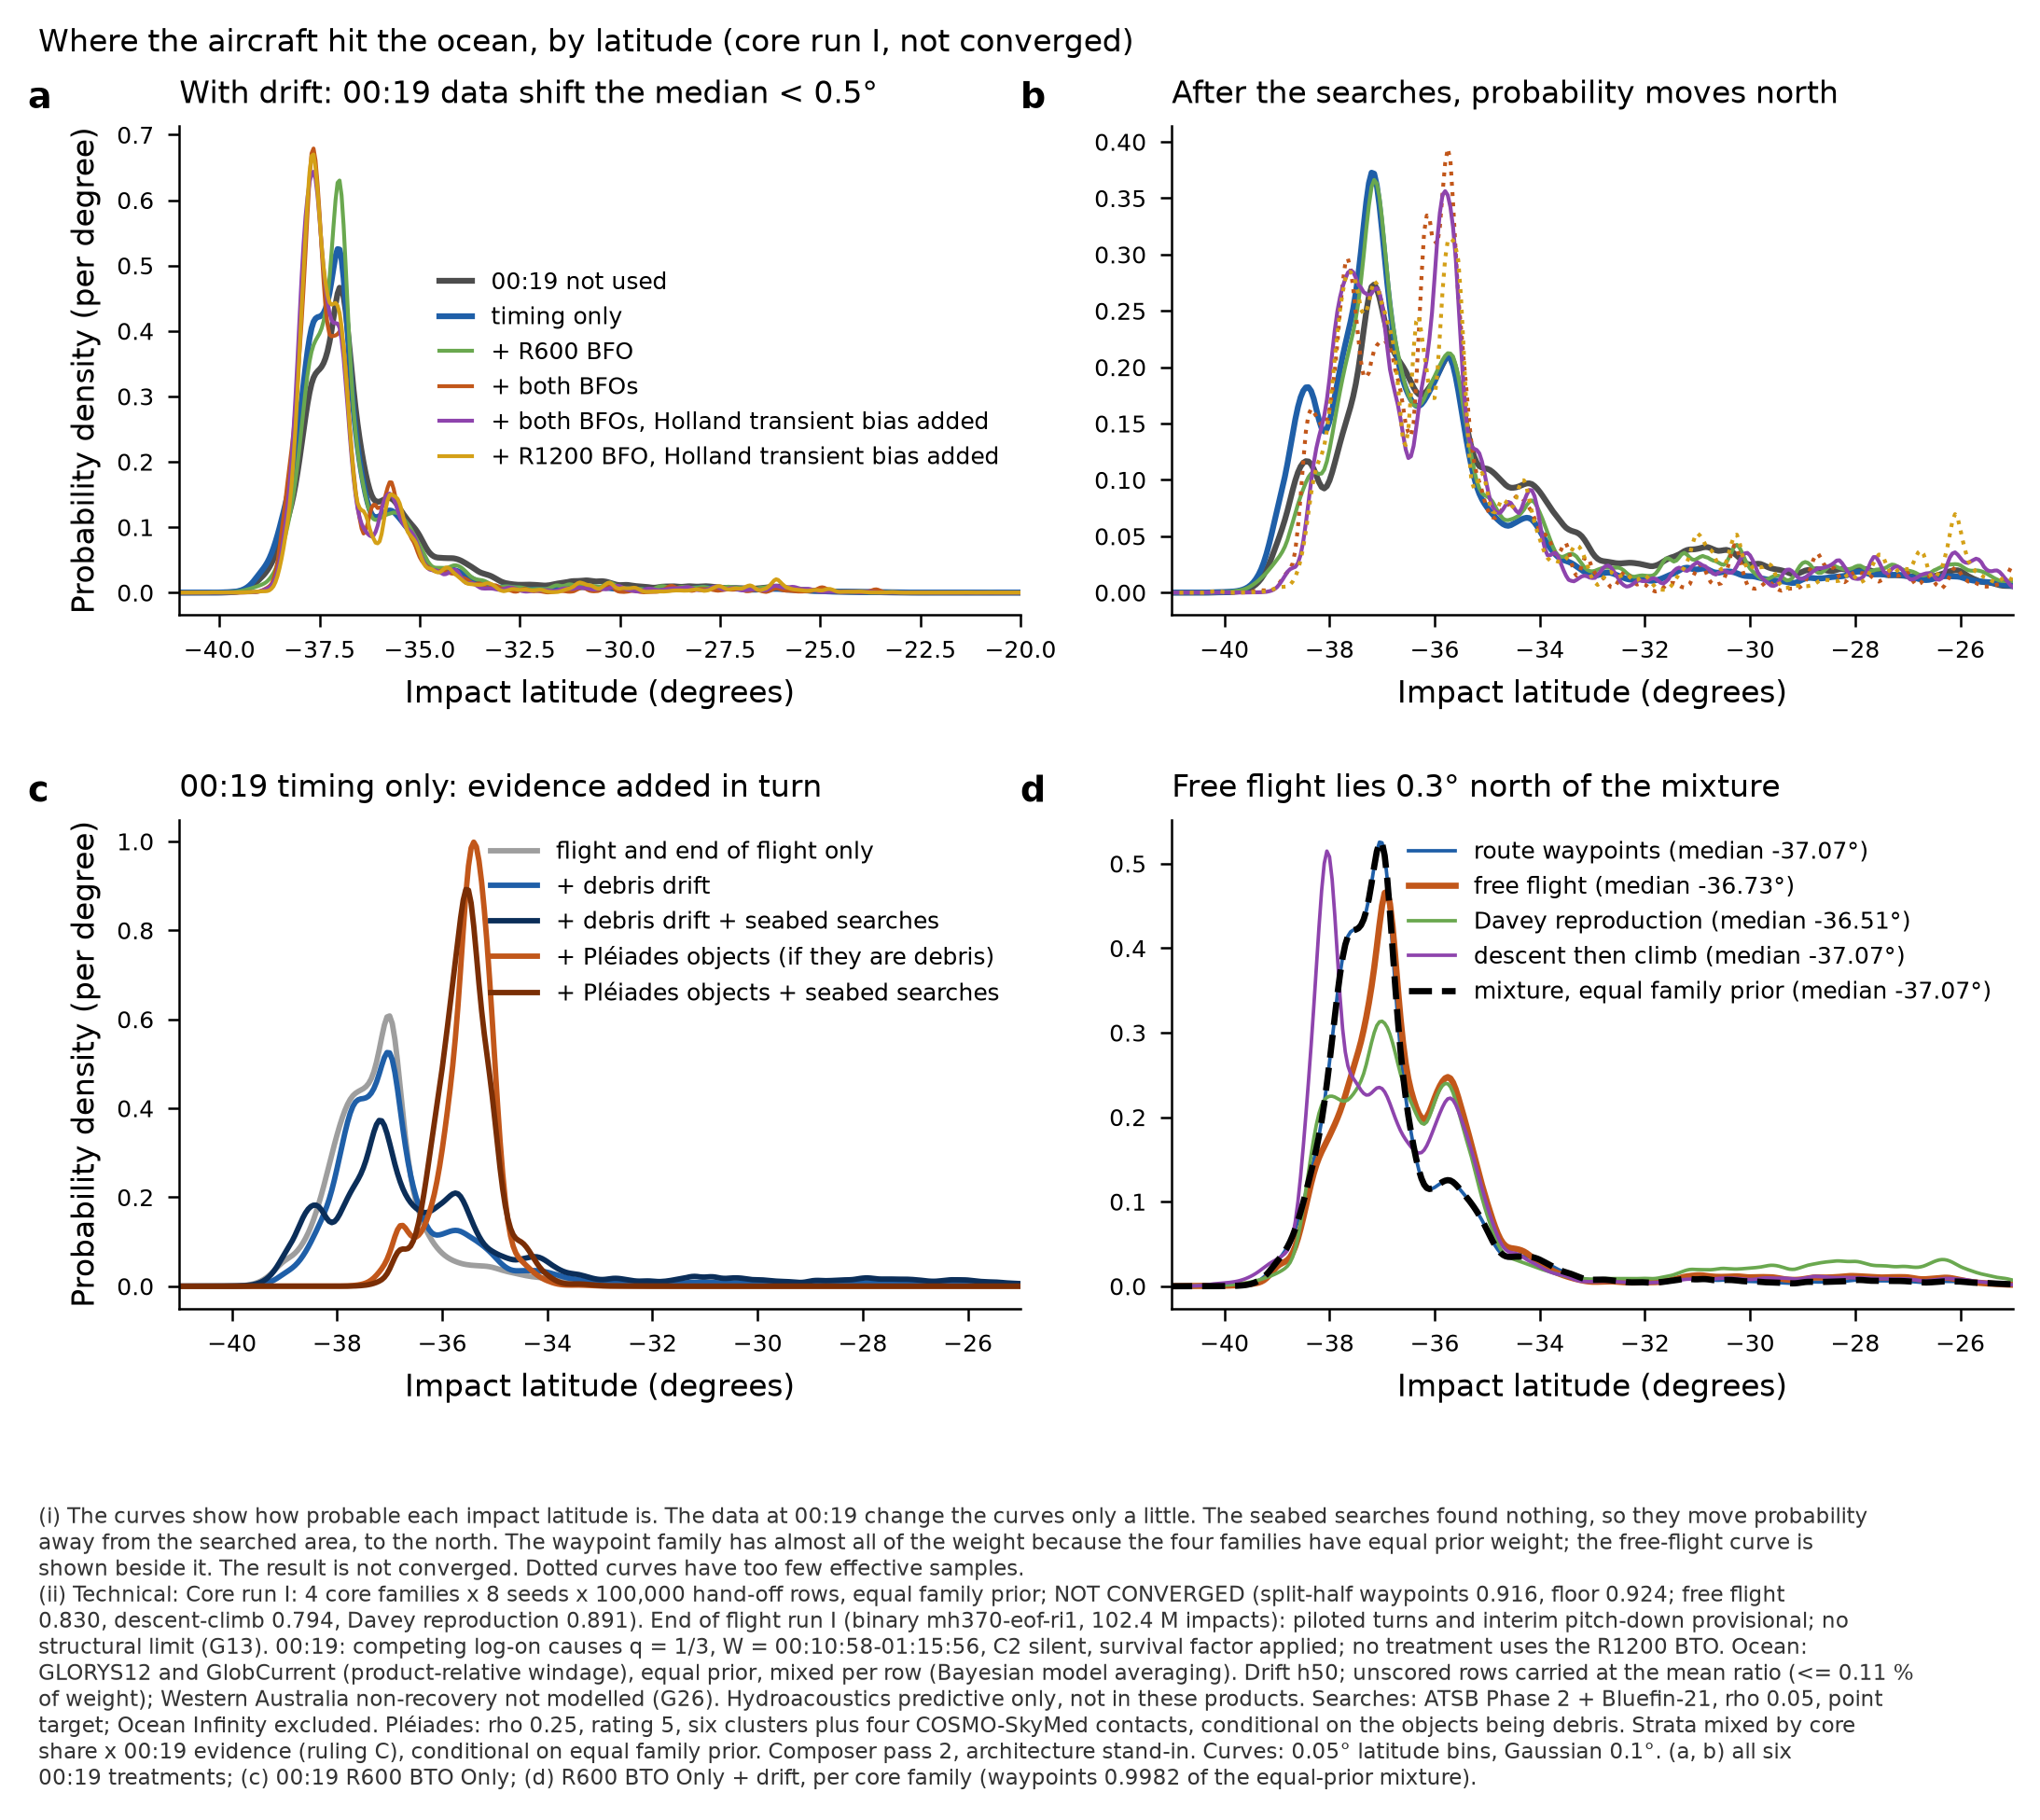
\includegraphics[width=\linewidth]{fig1-impact-latitude.png}

\caption{Impact arc-latitude distribution. (a) With the drift term, for all six treatments of the 00:19Z observations. (b) After the search term. (c) Evidence added in turn under the first burst timing offset alone. (d) Per route stratum, with the equal-prior mixture. Dotted curves have too few effective candidates to be quotable. Core run I, composed pass 2; not converged; conditional on an equal family prior.}

\end{figure}

% ALT TEXT for Figure 1 (required at submission): Four line charts of probability density against impact latitude from 41 to 20 degrees south. All four peak between 38 and 36 degrees south. In panel b the peak moves north and flattens after the search term is applied. In panel d the free-flight curve lies about 0.3 degrees north of the mixture.

Figure 1(a) shows the six treatments with the drift term applied, and Figure 1(b) the same six after the search term; the shift of the mode northward and the flattening of the distribution are visible in the second panel and are quantified in Section 3.6.

That cost determines what can be concluded. Before the search term is applied all six treatments are estimable, with effective sample sizes from 1,526 to 487,026. After it, the treatment using both frequency offsets as recorded falls to 393 effective candidates and the treatment correcting only the second offset to 610, both below the floor of 1,000; the treatment correcting both offsets remains just above it at 1,432. The two cells which correspond to the named hypotheses of Holland (2018) fall furthest: one from 275 effective candidates before composition to between 29 and 220 after it, the other from 833 to between 42 and 562.

The conclusion is therefore a negative one and is stated as such. With the sampler as it stands, the treatment of the 00:19Z observations which the evidence favours cannot be determined, and the apparent stability of the median across treatments is in part a statement about the sampler rather than about the observations. The uncertainty arising from the interpretation and use of the 00:19Z observations is therefore reported across all six treatments, in preference to selecting one of them.

\subsection{3.5.  Debris drift}

The drift term widens the impact distribution rather than narrowing it. Under the first burst timing offset alone the 90% region grows from 117,000km² to 165,000km² and shifts north-east, the median moving from −37.24° to −37.07° and the mean position from 37.08°S 90.31°E to 36.59°S 90.93°E. With the 00:19Z observations held out the widening is larger, from 152,000km² to 270,000km².

The drift evidence does not discriminate between the treatments of the 00:19Z observations: the change in log marginal likelihood on adding the term spans only 0.10 nats across all six, from −128.06 to −128.16. Nor does it select an ocean product. The posterior probability of the Copernicus reanalysis is 0.46 to 0.51 with drift alone, 0.47 to 0.51 after the search term and 0.54 to 0.63 when the imagery term is included, so the absolute log Bayes factor never exceeds 0.53. On this evidence the choice of global ocean reanalysis is not resolved by the debris, and the averaging of equation (10) is the correct treatment rather than a convenience.

\begin{figure}[htbp]\centering

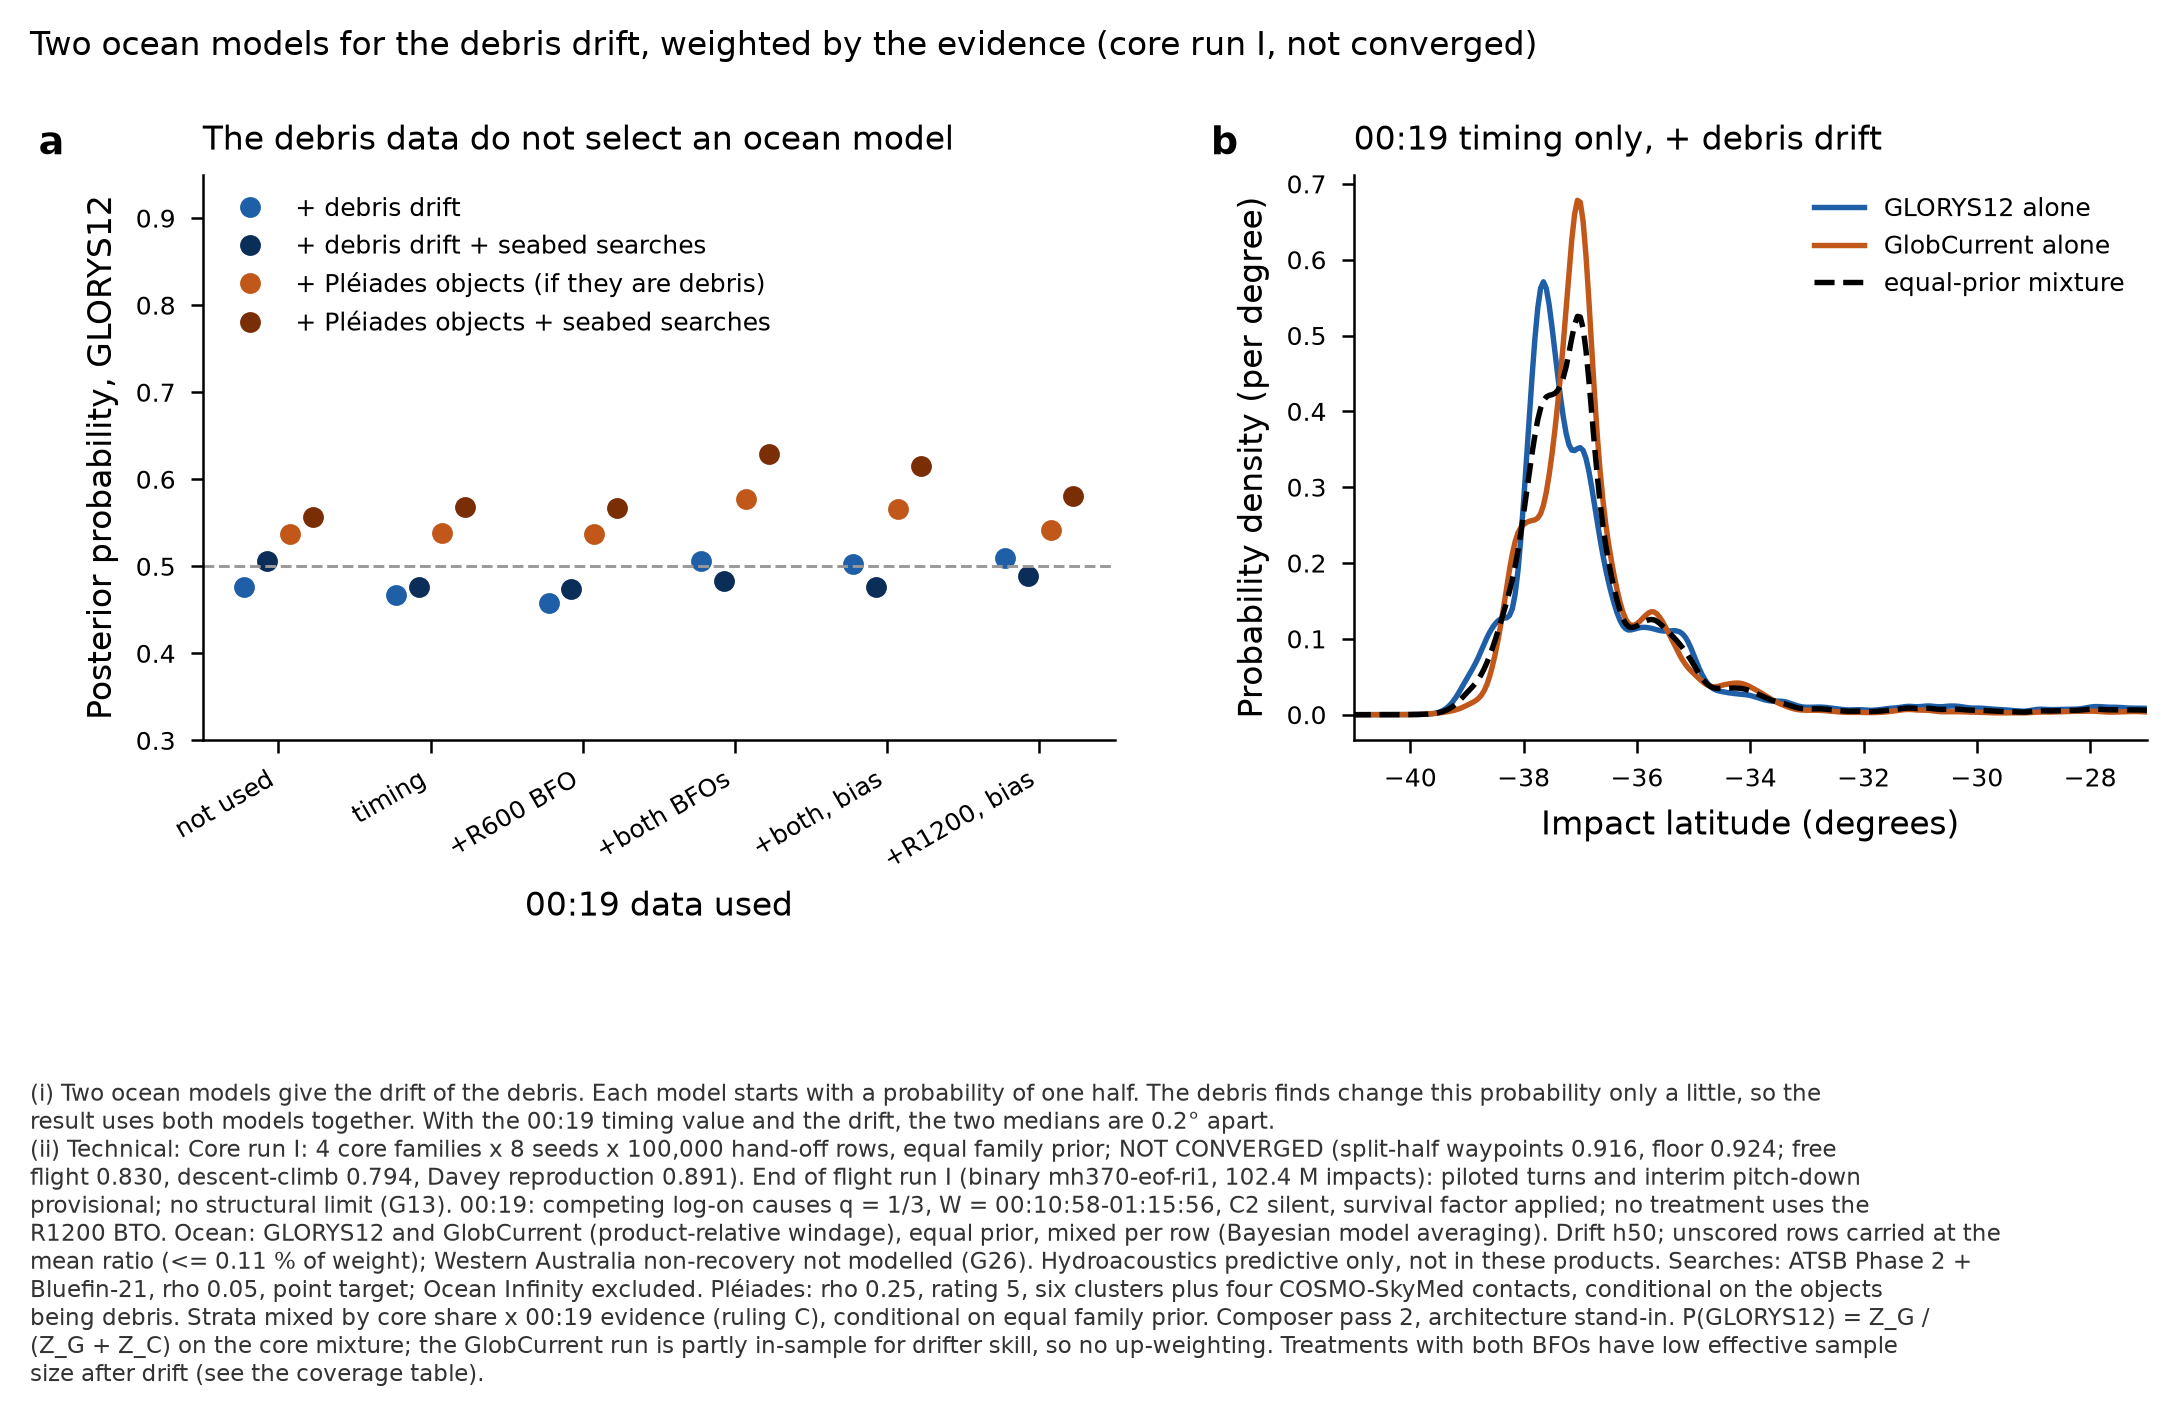
\includegraphics[width=\linewidth]{fig3-ocean-models.png}

\caption{Posterior probability of the first ocean product under each treatment of the 00:19Z observations and each composed product (a), and the impact arc-latitude distribution under each product separately with their equal-prior mixture (b). The dashed line in (a) marks the equal prior of one half. Not converged.}

\end{figure}

% ALT TEXT for Figure 2 (required at submission): Panel a is a dot plot of posterior probability between 0.3 and 0.9 against the six 00:19 treatments; all points lie between 0.45 and 0.63, close to the equal-prior line at 0.5. Panel b shows two single-product density curves about 0.2 degrees apart with their mixture between them.

Figure 2 shows that the posterior weight of either product stays close to the equal prior of one half under every treatment and every composed product, and that the two products give impact distributions whose medians differ by about 0.2°.

This result carries the label that the absence of recoveries on the Western Australian coast is not modelled, because the beaching geometry covers only the coastlines on which items were in fact recovered. That omission removes a line of disconfirming evidence which would act on precisely the impact locations towards which the search term moves probability, and it is the most consequential single omission in the study.

\subsection{3.6.  The unsuccessful searches}

The search term is the largest single factor acting on the impact distribution. It removes 54 to 71% of the probability mass, a change in log marginal likelihood of −0.78 to −1.23 nats, moves the median arc-latitude 0.3° to 1.2° north, and enlarges the 90% region by 60 to 96%: under the first burst timing offset alone, from 165,000km² to 309,000km², with the median moving from −37.07° to −36.76° and the 5th to 95th percentile range widening from −38.36° to −33.33° to −38.68° to −28.40°.

The direction is the informative part. A search which found nothing does not concentrate a distribution; it removes the places which were searched and redistributes the probability to places which were not, and here those lie north of and outside the searched corridor. The term also acts on the end-of-flight families, reducing the posterior probability of the unpiloted family A1 from 0.17 to 0.08 while the two piloted families gain, which follows because A1 terminates closest to the seventh arc and therefore within the best-searched ground.

\begin{figure}[htbp]\centering

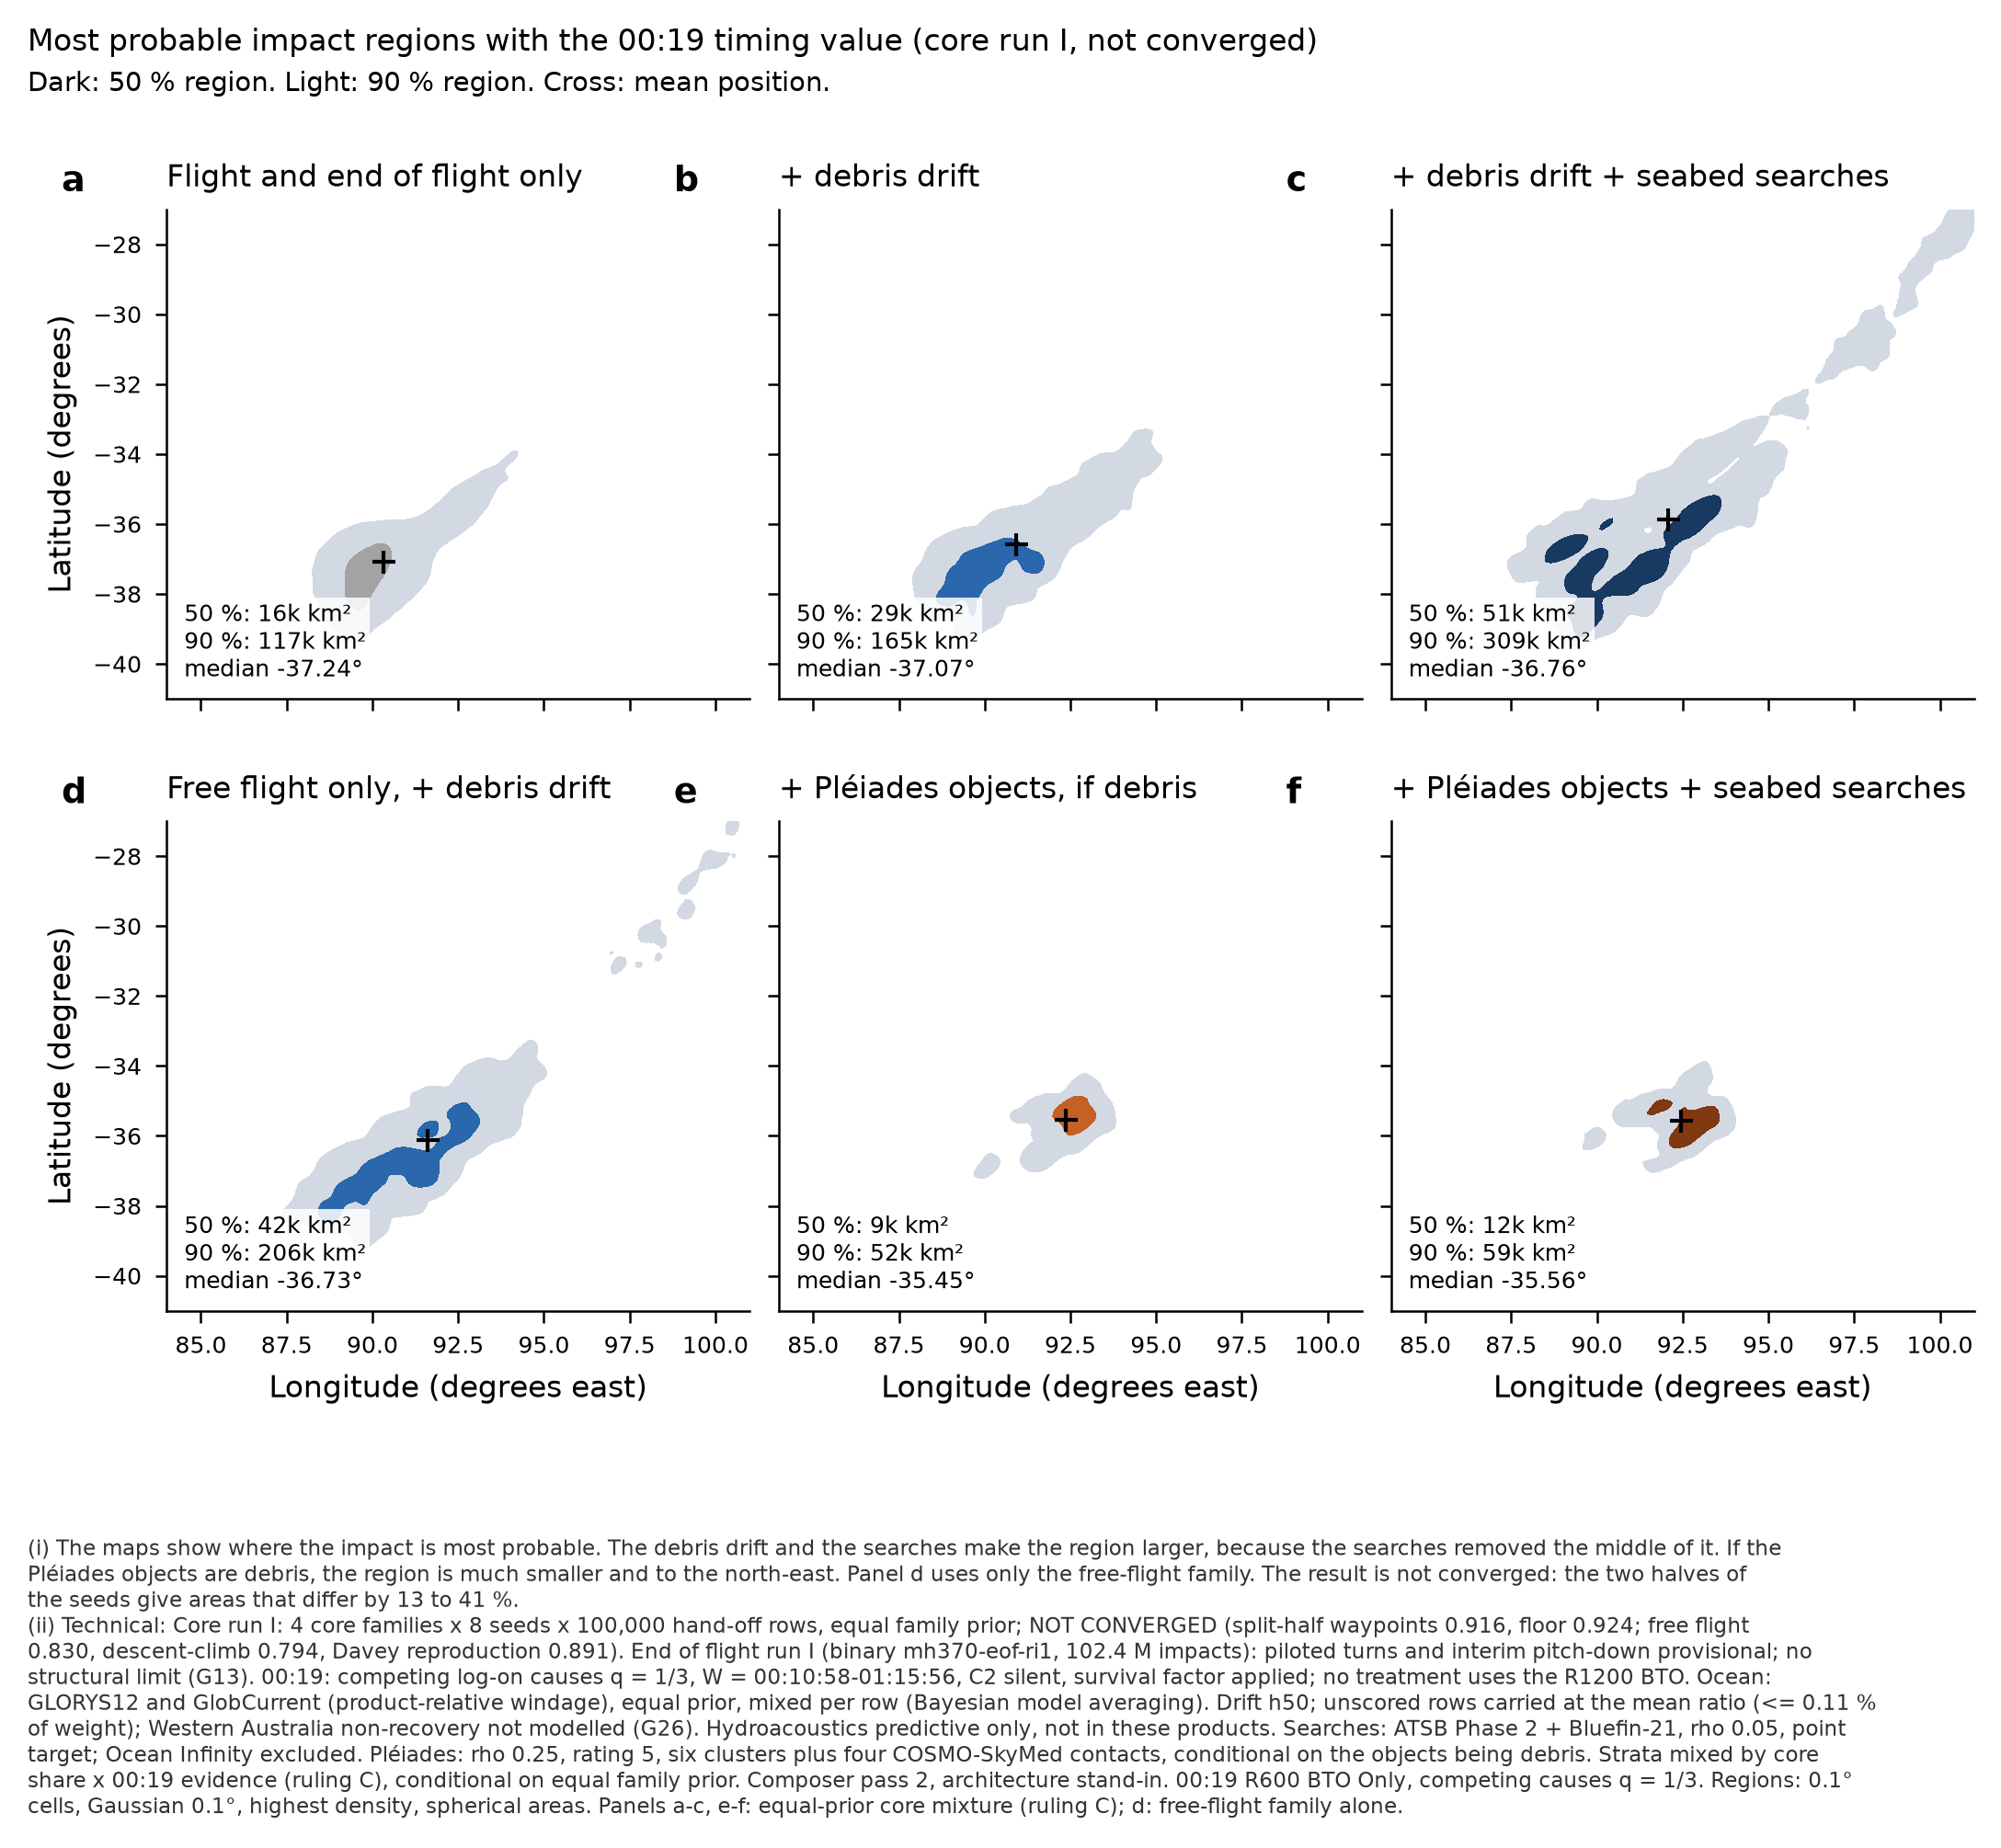
\includegraphics[width=\linewidth]{fig2-impact-regions.png}

\caption{Highest-density impact regions under the first burst timing offset alone. Dark: 50\% region. Light: 90\% region. Cross: mean position. (a) Flight and end of flight only. (b) With the drift term. (c) With the drift and search terms. (d) Free-flight stratum alone, with drift. (e), (f) With the imagery term, conditional on the imaged objects being debris from this aircraft. Not converged: the two halves of the replicate set give areas differing by 13 to 41\%.}

\end{figure}

% ALT TEXT for Figure 3 (required at submission): Six maps of latitude 27 to 41 degrees south against longitude 84 to 101 degrees east. The shaded region is a narrow band running south-west to north-east. It grows from panel a to panel c as the drift and search terms are added, and contracts markedly in panels e and f under the imagery hypothesis.

Figure 3 shows the effect as regions rather than as marginals: the 50% region grows from 16,000km² to 51,000km² and the band extends north-east along the arc as the drift and search terms are added in turn.

Two qualifications work in the same direction and are stated with the result: the detection parameter is evaluated at a single conservative value, which understates the strength of the term, and the most recent search operation is excluded from the coverage used here. The search term as reported is therefore a lower bound on its true effect.

\begin{table}[htbp]\centering\caption{Composed impact distribution before and after the search term, for three treatments of the 00:19Z observations. All rows: not converged; conditional on an equal family prior; Western Australia non-recovery not modelled; search detection parameter conservative and the most recent search operation excluded.}

\vspace{3pt}\small\begin{tabular}{@{}p{3.9cm}p{3.5cm}p{2.5cm}p{1.9cm}p{2.2cm}@{}}\toprule

00:19Z treatment & Product & Median φ\_imp (5-95\%) & 90\% area (km²) & ESS \\ \midrule

Held out & + drift & −36.86 (−38.24 to −30.60) & 270k & 374,577 \\

Held out & + drift + searches & −35.97 (−38.51 to −28.10) & 432k & 117,375 \\

R600 BTO only & + drift & −37.07 (−38.36 to −33.33) & 165k & 487,026 \\

R600 BTO only & + drift + searches & −36.76 (−38.68 to −28.40) & 309k & 158,101 \\

Both BFOs, Holland transient bias added & + drift & −37.29 (−38.14 to −33.64) & 96k & 7,098 \\

Both BFOs, Holland transient bias added & + drift + searches & −36.05 (−38.13 to −27.17) & 188k & 1,432 \\

\bottomrule\end{tabular}\end{table}

Table 3 gives the composed distribution before and after the search term for three of the six treatments. Two features of it are worth drawing out. The treatments which use the second frequency offset produce the tightest distribution before the search term is applied and the tightest after it, so the ordering of the treatments by precision survives composition even though, as Section 3.4 records, their effective sample sizes do not support a choice between them. And the proportional effect of the search term is largest where the prior distribution was tightest: the 90% region roughly doubles in every row, so the term does not merely trim the distribution's edges but redistributes its mass.

The effect on the end-of-flight families is consistent across treatments. Before the search term the three families carry posterior probabilities of approximately 0.17, 0.42 and 0.42 for the unpiloted, piloted-glide and continued-control families respectively; after it, 0.08, 0.47 and 0.45. The search term therefore acts as evidence about the manner of the end of flight and not only about position, which is a consequence of the integration: in a separated analysis the searched areas could not inform the end-of-flight family at all.

\subsection{3.7.  The imagery hypothesis, reported conditionally}

The satellite imagery term is evaluated as a likelihood on the shared impact samples and conditional on the imaged objects being debris from this aircraft, following the official analysis of the imagery (Minchin et al., 2017). It is never implemented as a selection of trajectories which could reach the imaged position, because selecting candidates by whether they reach a hypothesised outcome is not inference; the subset consistent with the hypothesis emerges instead as a posterior reweighting.

Under that condition the imagery term tightens the distribution substantially, the 90% seabed region falling to 70,300km² from 259,700km² under drift alone with the 00:19Z observations held out, and 76,600km² once the search term is also applied. It also raises the posterior probability of the Copernicus ocean reanalysis to between 0.54 and 0.63, which is the only point at which any term in the composition discriminates between the two ocean products, and even there the absolute log Bayes factor does not exceed 0.53. Every number in this subsection carries the condition that the imaged objects are debris from this aircraft; none of them is evidence that they are.

\subsection{3.8.  The seabed distribution}

The seabed distribution is obtained from the impact distribution by the sinking transform of Section 2.7. With the 00:19Z observations held out, the 90% region on the seabed is 151,700km² from the flight and end-of-flight stages alone, 259,700km² after the drift term and 409,800km² after the search term, with the median seabed latitude moving from −37.05° to −36.85° and then to −35.95°. The seabed regions coincide with the corresponding impact regions to within 2.5%, which is expected, since the horizontal displacement during the descent through the water column is small against the width of the impact distribution.

\begin{figure}[htbp]\centering

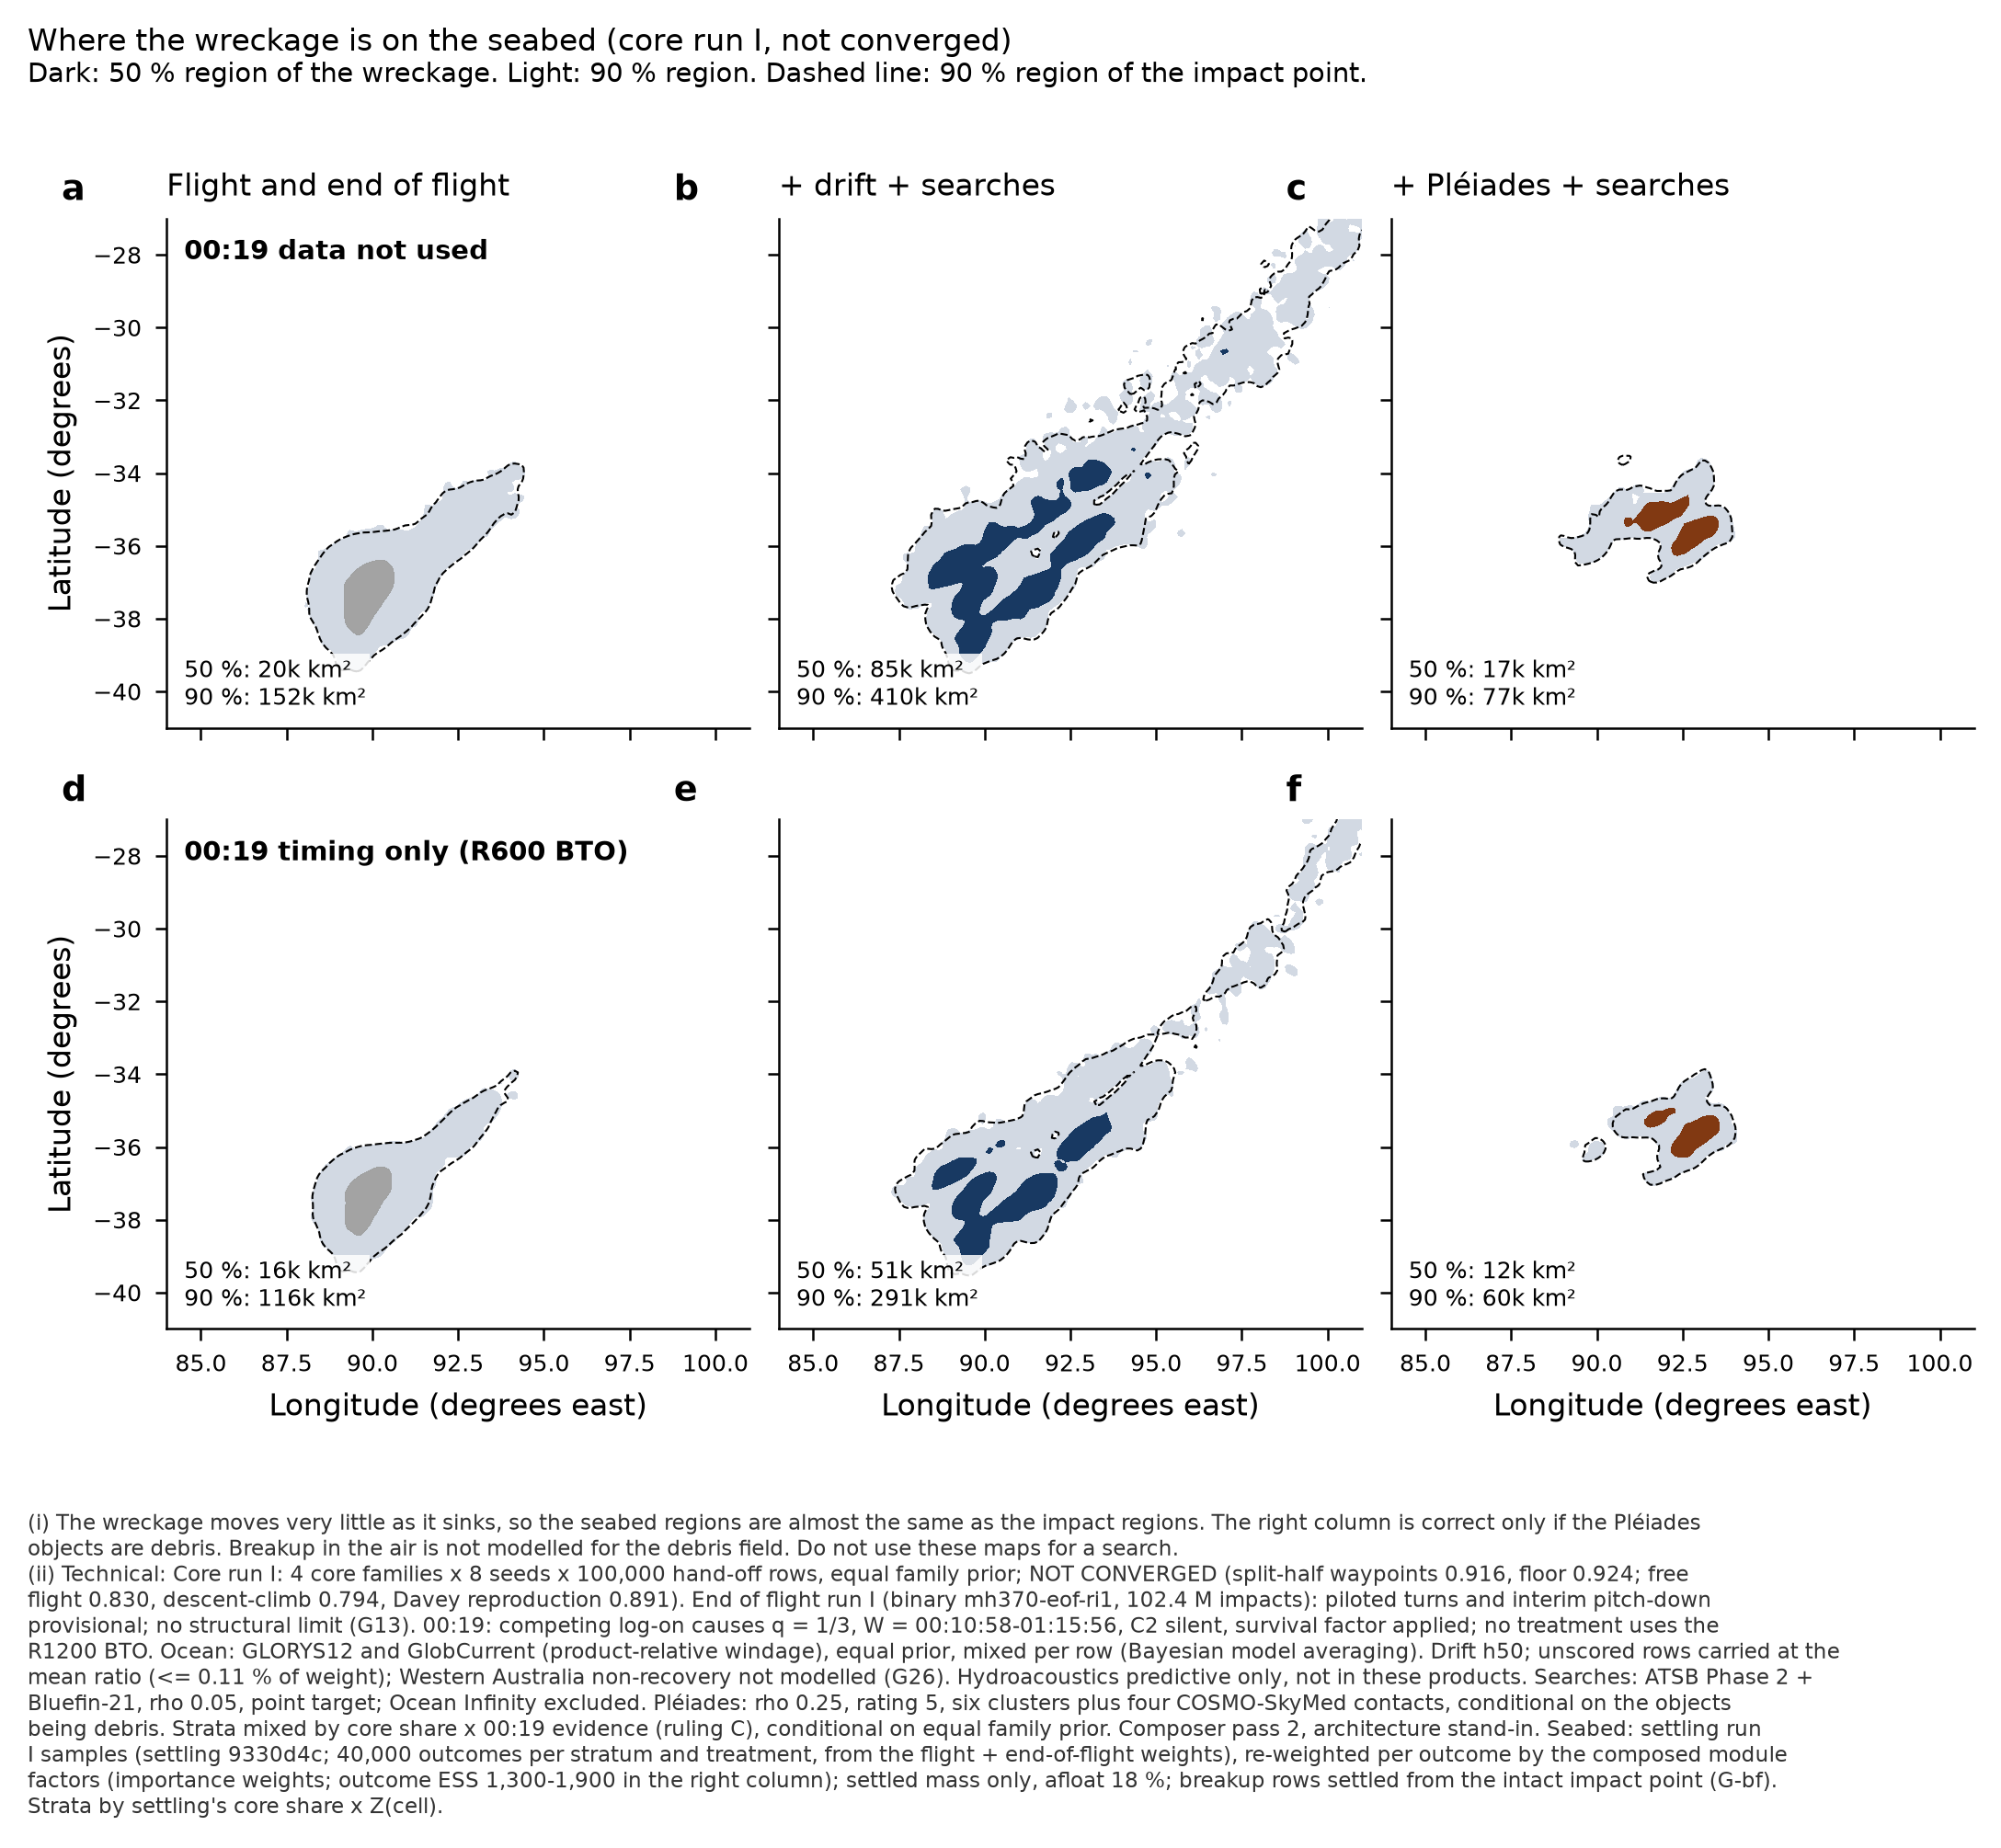
\includegraphics[width=\linewidth]{fig5-seabed.png}

\caption{Seabed regions for the wreckage field, with the 90\% impact region overlaid as a dashed outline. Dark: 50\% region. Light: 90\% region. Upper row: 00:19Z observations held out. Lower row: first burst timing offset only. Columns: flight and end of flight; with the drift and search terms; with the imagery and search terms. Breakup in the air is not modelled for the field, and these regions are not a search plan.}

\end{figure}

% ALT TEXT for Figure 4 (required at submission): Six maps on the same axes as Figure 3, each showing a shaded seabed region with a dashed outline of the impact region almost coincident with it, confirming that the wreckage moves little during the descent through the water column.

Figure 4 places the seabed regions against the impact regions they derive from; the dashed outline of the impact region is almost coincident with the seabed region in every panel.

The seabed distribution inherits the non-convergence of Section 3.1 and adds to it: the two halves of the replicate set differ by 22 to 43% in the area of the 90% region. It also carries two labels of its own. The seabed ensemble is re-weighted from the composed candidate weights rather than drawn from them, which is a partial treatment, and the breakup rows are settled from the intact impact point, so the extent of the wreckage field is a lower bound.

\subsection{3.9.  Hydroacoustic prediction}

The hydroacoustic term is predictive and not evidential, and its log-likelihood ratios lie within noise. The reason is calibration rather than physics, and five specific gaps are responsible. There is no near-surface calibration source of known spectrum, so the directivity of a seismic air-gun source cannot be separated from its coupling into the water column. The deep explosive source spectrum below the bubble frequency is unknown to between 4 and 17dB, because the standard source-level relations were established for charges at shallower depths than the available calibration shots. No frequency band below 16Hz is calibrated by any deep source, while the bands in which an impact marker would be expected lie below 12.5Hz. At one of the two southern stations the Chagos Bank blocks every modelled path from every candidate impact position, so a non-detection there carries no information at all. And at a bathymetric ridge which cuts the sound-channel axis the modelled transmission loss is 49 to 55dB too lossy, an error which two-dimensional propagation modelling does not remove.

The consequence is that the limit on the hydroacoustic test is its power and not its model. An unarrested rapid descent deposits of the order of several gigajoules at the surface, which is roughly an order of magnitude above the energy of the nearest reference event for which a calibrated near-surface recording exists. Were the transmission loss absolutely calibrated and the band below 16Hz characterised, the predicted signal level at the unobstructed stations would separate the end-of-flight families by a margin which the present calibration uncertainty masks entirely, and a confirmed non-detection would down-weight the most energetic descents.

\subsection{3.10.  Evidence accounting}

Because the impact-level factors are selectable, each line of evidence can be costed in two currencies, the change it makes to the log marginal likelihood and the effective sample size it leaves behind, and the two do not move together. The search term changes ln p(z) by only −0.78 to −1.23 nats while removing most of the probability mass and reshaping the distribution substantially. The drift term sits at approximately −128 nats, which reflects the improbability of the observed recovery pattern under any impact position rather than discrimination between positions; the spread of that figure across the six treatments of the 00:19Z observations is only 0.10 nats, and it is the spread and not the level which carries information. Reporting the level alone would invite the reading that drift is the dominant evidence, when it is in fact the least discriminating term in the composition.

Effective sample size gives the other half of the accounting. Under the treatment using the first burst timing offset with the first frequency offset, the composition retains of the order of 6×10⁴ effective candidates after the flight and end-of-flight stages, 4×10⁴ after the drift term and 1×10⁴ after the search term, falling to a few thousand under the imagery hypothesis; that chain remains estimable throughout. The treatments using both frequency offsets do not, for the reasons given in Section 3.4. One line of evidence is therefore capable of rendering another unquotable, which is why the effective sample size is reported per factor beside every number rather than once for the composition as a whole.

\begin{figure}[htbp]\centering

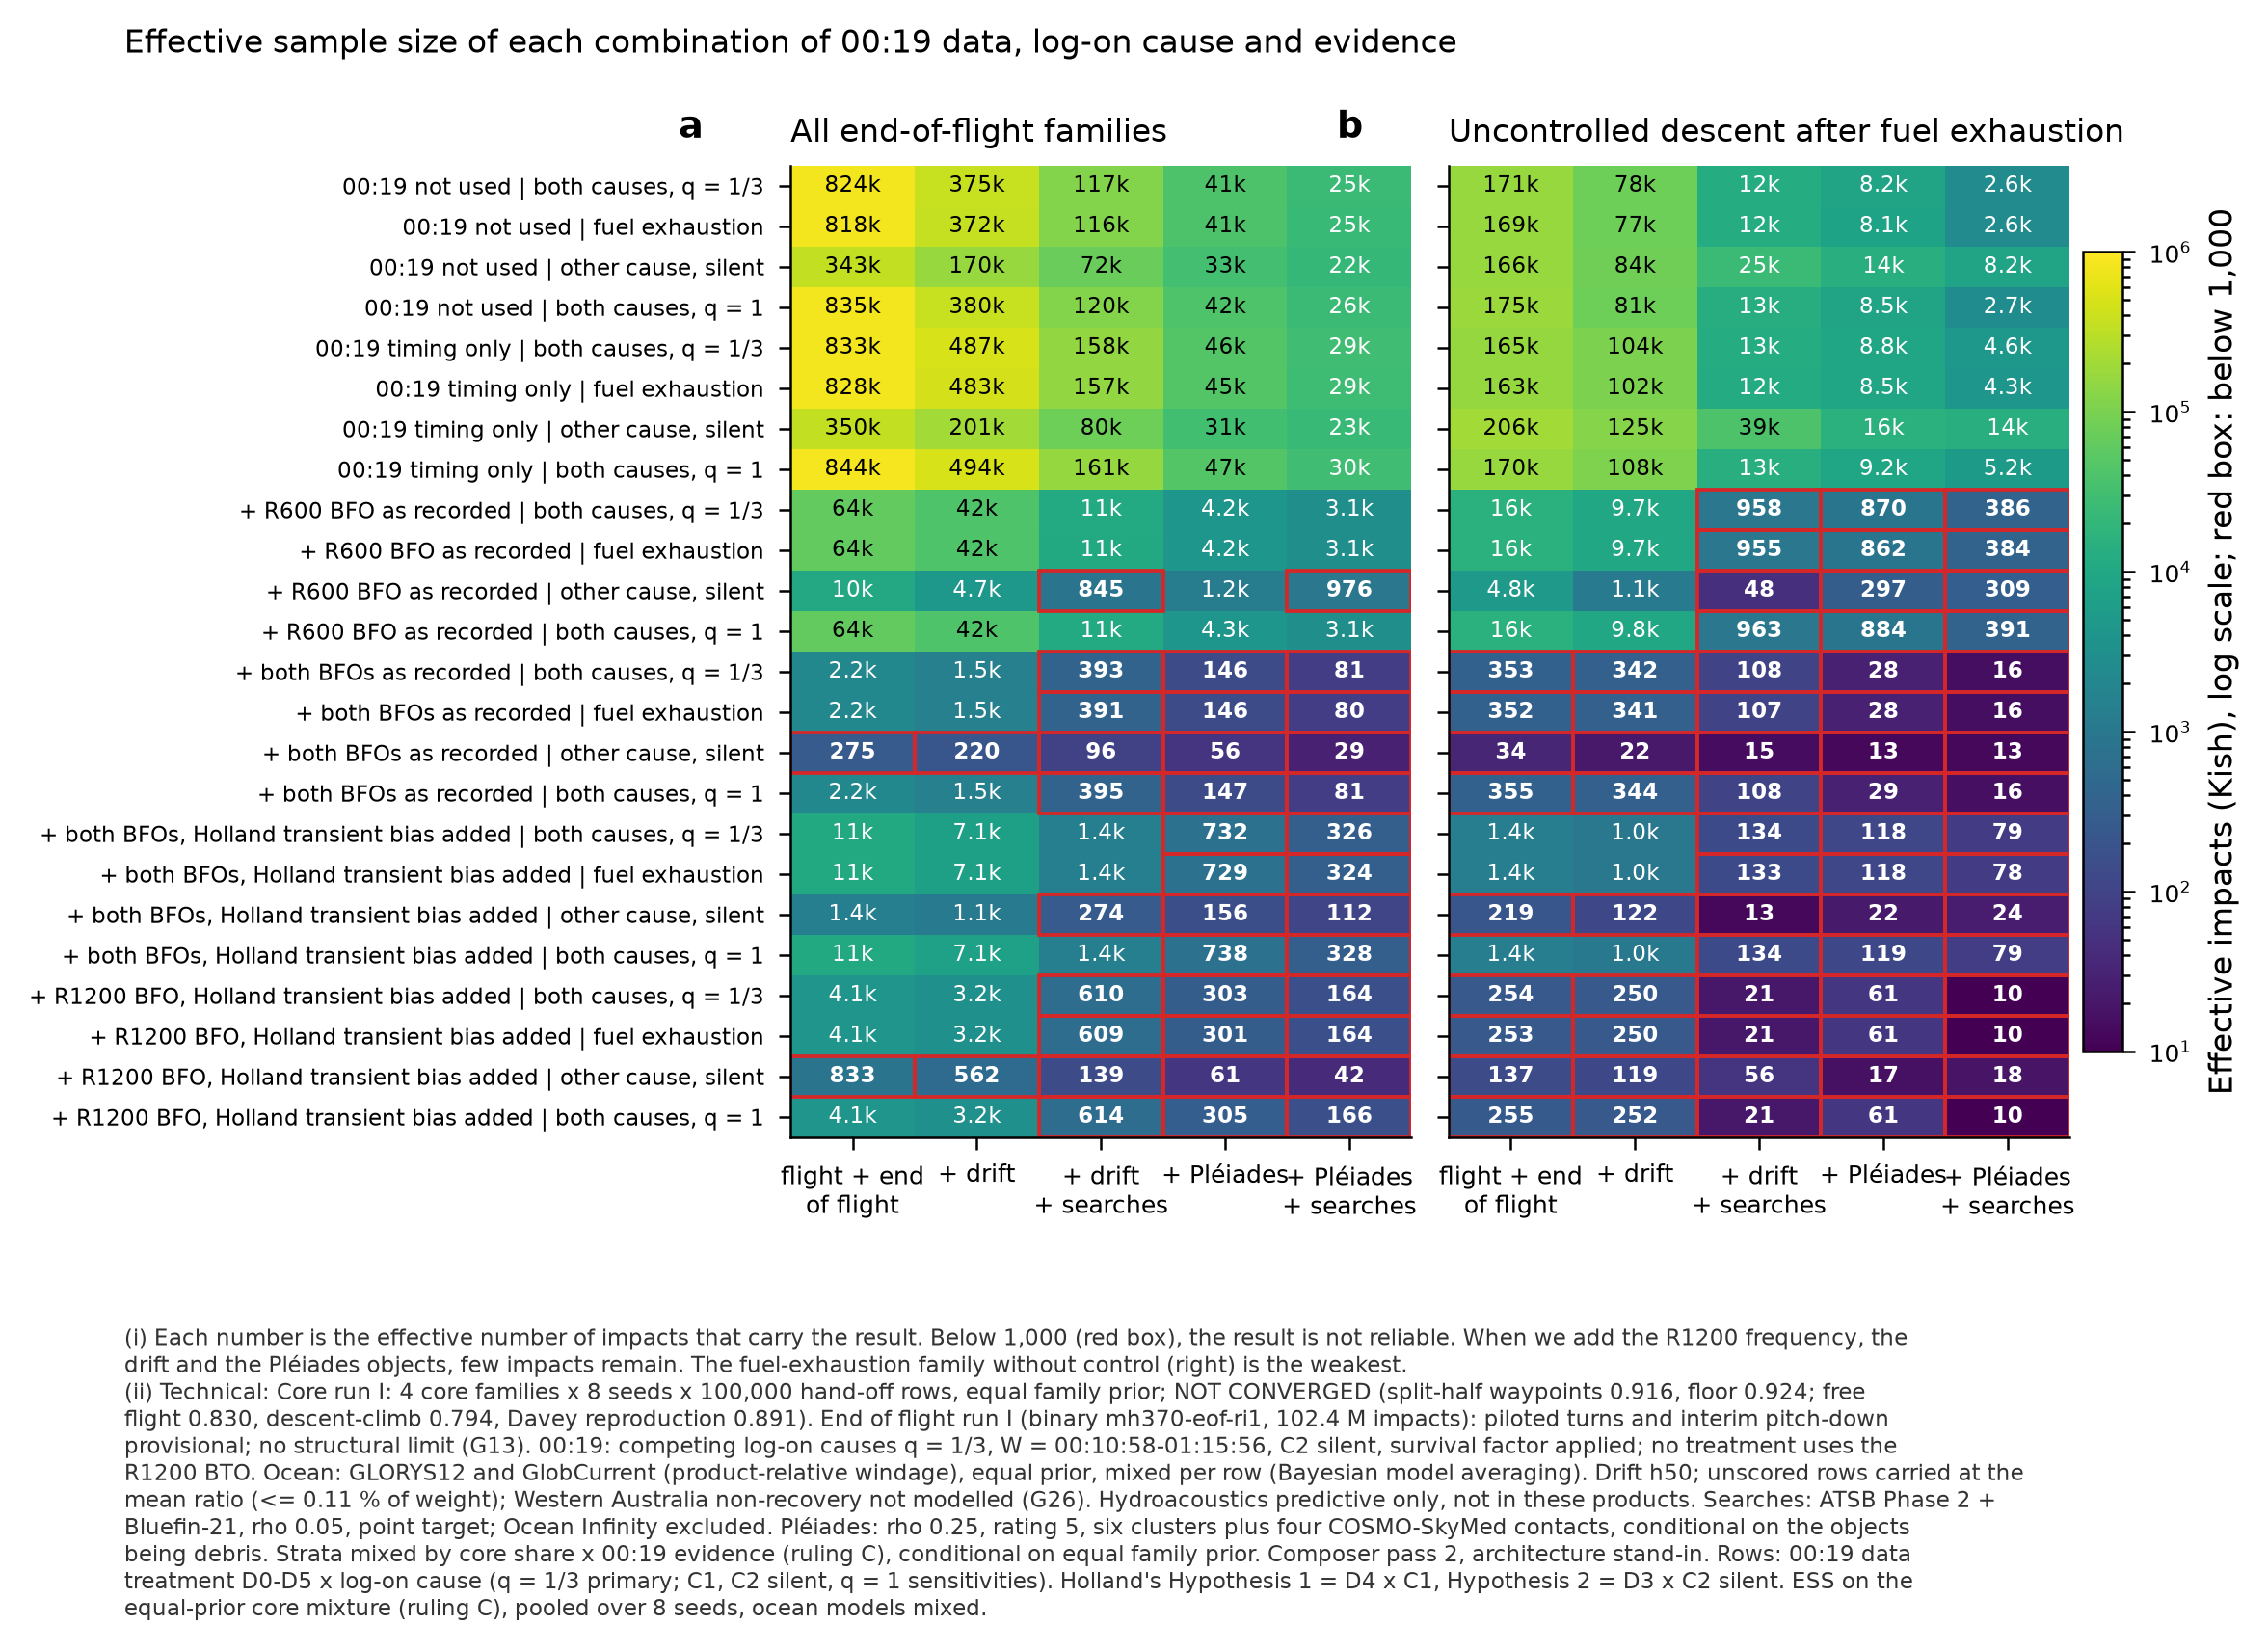
\includegraphics[width=\linewidth]{fig4-coverage-ess.png}

\caption{Effective sample size for every combination of 00:19Z data treatment, assumed cause of the power interruption and composed evidence product, for all end-of-flight families (a) and for the unpiloted family alone (b). Values below 1,000, outlined, are not estimable. Note the logarithmic scale.}

\end{figure}

% ALT TEXT for Figure 5 (required at submission): Two heat-map tables of effective sample size on a logarithmic scale from ten to one million. Values fall from several hundred thousand in the leftmost column to tens in the rightmost. Cells below one thousand, concentrated in the lower right of both panels, are outlined.

Figure 5 gives the effective sample size of every cell, and is the diagnostic on which the estimability statements of Sections 3.4 and 3.9 rest: the values fall by four orders of magnitude from left to right across the composition.

One accounting check closes a gap which was open at the previous composed pass. The candidates for which the drift term could not be computed amount to at most 0.11% of the base weight in any stratum and treatment, and excluding them changes ln p(z) by less than 0.001 and moves no median or area visibly. At the previous pass that uncomputed fraction was large enough that whether it was carried or excluded changed the composed areas materially; it no longer is, and the difference is a property of the run rather than of the composition.

\subsection{3.11.  Two negative results}

The published cruise state carries no vertical rate, and the omission appeared likely to matter, since the 184Hz step between the two frequency offsets at 00:19Z corresponds to an equivalent vertical rate of approximately 10,500ft/min, some nine times the largest bias excursion in the published work. Adding a vertical rate to the cruise state changes the posterior median by 0.03° or less and the probability of the secondary mode by about two percentage points. The omission is an order of magnitude larger than the noise against which it was being judged, and it is nevertheless not a lever on the secondary mode, because the altitude changes it represents are too brief.

Four of the five sampler interventions attempted failed to improve replicate agreement, and all four remain runnable behind configuration flags. The one which succeeded did so by aiming the proposal at the cells in which the end-of-flight families separate, rather than by adding candidates. The pattern across the five is that the difficulty of this posterior is a structural multi-modality and not a shortage of samples, which is why the recommendation of Section 4 is a sampler and not more compute.

\section{4.  CONCLUSIONS AND RECOMMENDATIONS}

An integrated Bayesian reconstruction of the loss of MH370 has been built and run. One probability distribution is carried from the last radar fix at 18:01Z through the satellite handshakes to 00:11Z, through a simulated end of flight to water impact, and through the descent of the wreckage to the seabed, and is weighted by the drift of the recovered debris, by the unsuccessful searches, by satellite imagery and by hydroacoustic prediction on one shared set of impact samples.

Four substantive conclusions follow, each under the labels of Section 3.1. The waypoint route family carries 0.998 of the posterior weight within the core mixture, against 0.0011 for free flight, which is evidence that the satellite observations are explained very much better by trajectories tracking published navigation fixes than by trajectories wandering under the published manoeuvre model, among the strata built and subject to the turn model stated. The unsuccessful seabed searches are the largest single factor acting on the impact distribution, removing 54 to 71% of the probability, moving the median arc-latitude 0.3° to 1.2° north and enlarging the 90% region by 60 to 96%, and reducing the posterior probability of the unpiloted end-of-flight family from 0.17 to 0.08. The drift of the recovered debris widens the distribution rather than narrowing it and discriminates neither between the treatments of the 00:19Z observations nor between global ocean reanalyses. And the hydroacoustic record is at present predictive only, its log-likelihood ratios lying within noise for reasons of calibration.

The fifth conclusion is that none of these distributions is converged against the replicate-agreement criterion proposed in equation (14). The orderings and the directions of effect are stable across replicate partitions; the areas and the medians are not. This is reported as a result because the alternative, quoting areas to three significant figures from an unconverged run, would be worse than quoting nothing.

Four lines of further work follow, ordered by how much each would change the answer rather than by how difficult each would be. First, a sampler aimed at the cells in which the end-of-flight families separate, which is the binding constraint on every number reported here and which Section 3.9 indicates will not be resolved by additional compute. Second, an end-of-flight model which reaches the rapid descents that the 00:19Z frequency offsets admit, together with a structural limit which excludes the impact speeds the present model allows, since 11 to 21% of the composed weight lies above 1.25 times the maximum operating speed before the search term is applied. Third, the Western Australian non-recovery term, which would act directly on the region towards which the search term moves probability. Fourth, absolute calibration of the hydroacoustic transmission loss together with characterisation of the band below 16Hz: of the four this is the only one which could convert an unused observation into a decisive one, and its value of information is correspondingly the largest.

\section{REFERENCES}

\begingroup\small

Ashton, C., Shuster Bruce, A., Colledge, G. and Dickinson, M. (2015). The Search for MH370. The Journal of Navigation, 68, 1-22. https://doi.org/10.1017/S037346331400068X.\par\medskip

Davey, S., Gordon, N., Holland, I., Rutten, M. and Williams, J. (2016). Bayesian Methods in the Search for MH370. Springer. https://doi.org/10.1007/978-981-10-0379-0.\par\medskip

Holland, I. D. (2018). MH370 Burst Frequency Offset Analysis and Implications on Descent Rate at End-of-Flight. IEEE Aerospace and Electronic Systems Magazine, 33, 24-33. https://doi.org/10.1109/MAES.2018.170048.\par\medskip

Lellouche, J.-M., Greiner, E., Bourdalle-Badie, R. and others (2021). The Copernicus Global 1/12 degree Oceanic and Sea Ice GLORYS12 Reanalysis. Frontiers in Earth Science, 9, 698876. https://doi.org/10.3389/feart.2021.698876. [AUTHOR LIST TO BE COMPLETED]\par\medskip

Minchin, S., Mueller, N., Lewis, A., Byrne, G. and Tran, M. (2017). Summary of imagery analyses for non-natural objects in support of the search for Flight MH370: Results from the analysis of imagery from the PLEIADES 1A satellite undertaken by Geoscience Australia. Geoscience Australia, Record 2017/013. https://doi.org/10.11636/record.2017.013.\par\medskip

Ng, H.-F., Zhong, Y., Groves, P. D. and Hsu, L.-T. (2024). Grid-based 3DMA GNSS with clustering and Doppler velocity. The Journal of Navigation, 77, 658-676. [VERIFY DOI]\par\medskip

Stone, L. D., Keller, C. M., Kratzke, T. M. and Strumpfer, J. P. (2014). Search for the Wreckage of Air France Flight AF 447. Statistical Science, 29, 69-80. https://doi.org/10.1214/13-STS420.\par\medskip

\endgroup

\section{ACKNOWLEDGEMENTS}

[To be completed. The journal itself must not be acknowledged.]

\section{COMPETING INTERESTS}

Competing interests: The author declares none.

\section{USE OF ARTIFICIAL INTELLIGENCE TOOLS}

[To be completed, and required by the journal. A declaration must describe any artificial intelligence tool used to generate text or images, or to analyse or extract insights from data, giving the tool name and version, the dates of use, how others may access it and a full description of the use; analysis use is declared in the methodology rather than in an acknowledgement. The estimator was developed and run with such assistance throughout, and the declaration must be assembled from what the repository records. See paper/JON-RULES.md section 7.]

\end{document}
